\documentclass{article}


\usepackage{xltxtra} % Loads fontspec, xunicode, metalogo, fxltx2e, and some extra customizations for XeLaTeX
%\defaultfontfeatures{Mapping=2.5tex-text} % to support TeX conventions like ``---''
\defaultfontfeatures{Mapping=2.5tex-text}
\setmainfont{Cambria}
\usepackage{csquotes}
\usepackage{graphicx}
\usepackage[margin=2.5cm]{geometry}
\newcounter{framenumber}
\setcounter{framenumber}{0}
%This command numbers frames and adds two blank lines for annotation.
\newcommand{\Annotate}{\stepcounter{framenumber}[\arabic{framenumber}]
\rule{\linewidth}{1pt}\\
\rule{\linewidth}{1pt}
\vspace{2\baselineskip}
\vfill
}
%Toggle to display subtitles in a different language
%\newcommand{\Bislama}[1]{#1}
\newcommand{\Bislama}[1]{}
\newcommand{\English}[1]{}
%\newcommand{\English}[1]{}

\begin{document}
\center 
{\huge Maṉḏa yirun'yirunha} 
\vfill

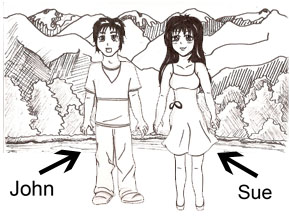
\includegraphics[scale=2.5]{OTL01}

\Bislama{Hemia Mary, hemia Lisa. Tufala i fren.}
\English{This is Mary, this is Lisa. The two are friends.}

\Annotate

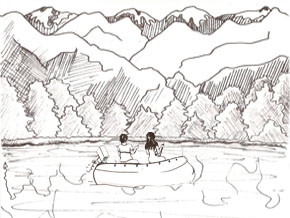
\includegraphics[scale=2.5]{OTL02}

\Bislama{Hemia Ros, mo hemia Christine. Tufala tu i fren blong Mary mo Lisa.}
\English{This is Rose and this is Christine. The two are friends with Mary and Lisa.}

\Annotate

\pagebreak

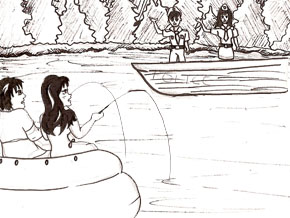
\includegraphics[scale=2.5]{OTL03}

\Bislama{Olgeta wuman oli go blong wok long garen.}
\English{The women go to work in the garden.}

\Annotate

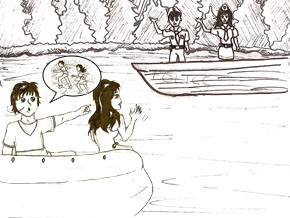
\includegraphics[scale=2.5]{OTL04}

\Bislama{Olgeta wuman oli go blong wok long garen.}
\English{The women go to work in the garden.}

\Annotate

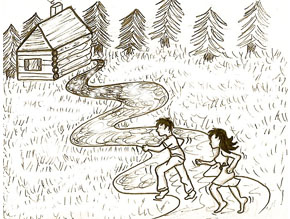
\includegraphics[scale=2.5]{OTL05.jpg}

\Bislama{Everi wan i stap wok long garen nao.}
\English{Everyone is busy working in the garden.}

\Annotate

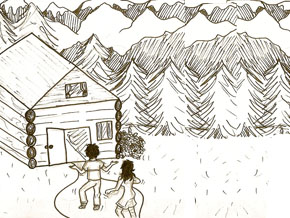
\includegraphics[scale=2.5]{OTL06.jpg}

\Bislama{Oli wok gogo, afta oli sidaon blong spel.}
\English{After a while, they sit down to rest.}

\Annotate

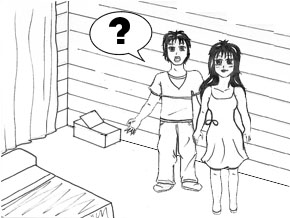
\includegraphics[scale=2.5]{OTL07.jpg}

\Bislama{Oli spel gogo, stap kakae, ale Christine i go long bus.}
\English{They rest a little and then Christine goes to the bush [to pee].}

\Annotate

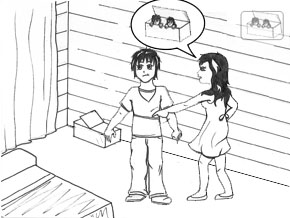
\includegraphics[scale=2.5]{OTL08.jpg}

\Bislama{Ale, Ros tu hemi go long bus.}
\English{Then, Rose also goes into the bush.}

\Annotate

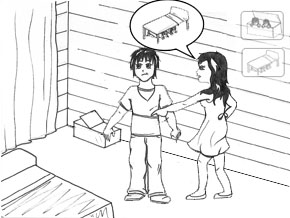
\includegraphics[scale=2.5]{OTL09.jpg}

\Bislama{Spel gogo, ale Mary wetem Lisa tufala i go bak long garen.}
\English{After a while, Mary and Lisa go back to the garden.}

\Annotate

\pagebreak

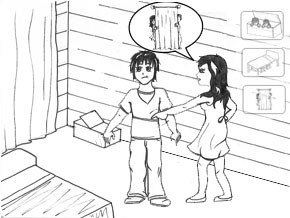
\includegraphics[scale=2.5]{OTL10.jpg}

\Bislama{Be taem tufala i kam bak, tufala i luk se wan red yam we Mary hemi bin plantem, hemi lus.}
\English{When they come back, they see that a red yam that Mary has planted is gone.}

\Annotate

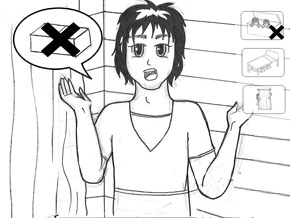
\includegraphics[scale=2.5]{OTL11.jpg}

\Bislama{Mary hemi askem Lisa: \enquote{Huia i kakae red yam blong mi?}}
\English{Mary asks Lisa: \enquote{Who has eaten my red yam?}}

\Annotate

\pagebreak

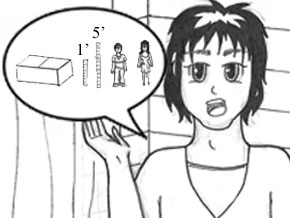
\includegraphics[scale=2.5]{OTL12.jpg}

\Bislama{Lisa hemi se: \enquote{Maet Christine i kakae, o maet i Ros.}}
\English{Lisa says: \enquote{It might have been Christine, or it might have been Rose.}}

\Annotate

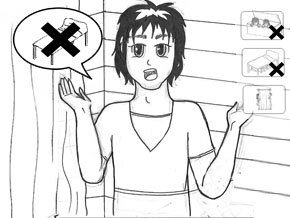
\includegraphics[scale=2.5]{OTL13.jpg}

\Bislama{Be Mary hemi se: \enquote{No, i no save i Ros. I mas Christine nomo hemi bin kakae red yam blong mi.}}
\English{But Mary says: \enquote{No, it can't have been Rose. It must have been Christine who ate my red yam}}

\Annotate

\pagebreak

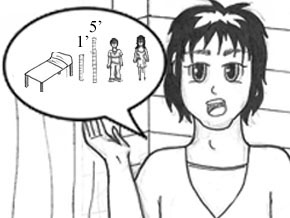
\includegraphics[scale=2.5]{OTL14.jpg}

\Bislama{Ale Lisa hemi se: \enquote{Bae yu lukluk tut blong Christine.}}
\English{So Lisa says: \enquote{Look at Christine's teeth.}}

\Annotate


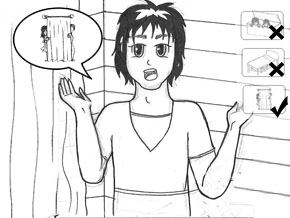
\includegraphics[scale=2.5]{OTL16.jpg}

\Bislama{Ale Mary hemi go long Christine, hemi kros long hem.}
\English{So Mary goes to Christine and is mad at her.}

\Annotate

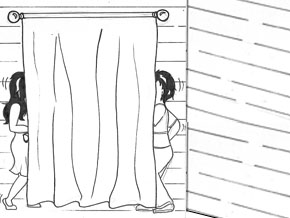
\includegraphics[scale=2.5]{OTL17.jpg}

\Bislama{Mary hemi se long Christine: \enquote{Yu kakae red yam blong mi!}}
\English{Mary says: \enquote{Christine, you ate my red yam!}}

\Annotate
\pagebreak

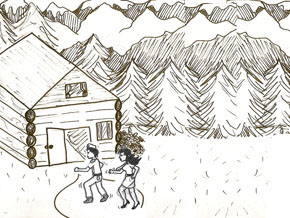
\includegraphics[scale=2.5]{OTL18.jpg}

\Bislama{Afta we Mary hemi talem olsem, Ros hemi stat blong laf.}
\English{After Mary has said this, Rose starts to laugh.}

\Annotate

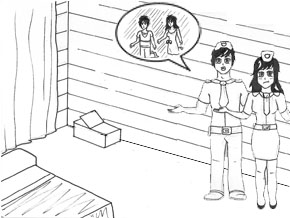
\includegraphics[scale=2.5]{OTL19.jpg}

\Bislama{Lisa hemi poentem Ros hemi se: \enquote{Yu luk, tut blong Ros i red!}}
\English{Lisa points at Rose and says: \enquote{Look, Rose's teeth are red!}}

\Annotate
\pagebreak

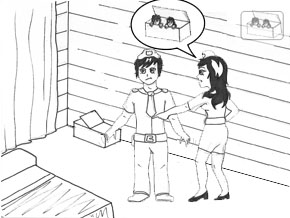
\includegraphics[scale=2.5]{OTL20.jpg}

\Bislama{Ale Lisa hemi se: \enquote{Christine hemi no bin kakae red yam blong yu, Mary! Ros nomo hemi spoilem yu!}}
\English{Then she says: \enquote{Christine didn't eat your red yam! It was Rose!}}

\Annotate

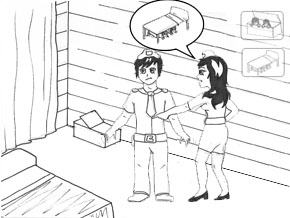
\includegraphics[scale=2.5]{OTL21.jpg}

\Bislama{Ale Lisa hemi se: \enquote{Christine hemi no bin kakae red yam blong yu, Mary! Ros nomo hemi spoilem yu!}}
\English{Then she says: \enquote{Christine didn't eat your red yam! It was Rose!}}

\Annotate
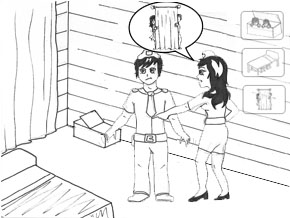
\includegraphics[scale=2.5]{OTL22.jpg}

\Bislama{Ale Lisa hemi se: \enquote{Christine hemi no bin kakae red yam blong yu, Mary! Ros nomo hemi spoilem yu!}}
\English{Then she says: \enquote{Christine didn't eat your red yam! It was Rose!}}

\Annotate
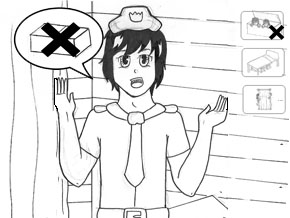
\includegraphics[scale=2.5]{OTL23.jpg}

\Bislama{Ale Lisa hemi se: \enquote{Christine hemi no bin kakae red yam blong yu, Mary! Ros nomo hemi spoilem yu!}}
\English{Then she says: \enquote{Christine didn't eat your red yam! It was Rose!}}

\Annotate
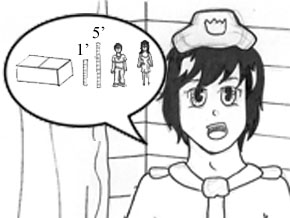
\includegraphics[scale=2.5]{OTL24.jpg}

\Bislama{Ale Lisa hemi se: \enquote{Christine hemi no bin kakae red yam blong yu, Mary! Ros nomo hemi spoilem yu!}}
\English{Then she says: \enquote{Christine didn't eat your red yam! It was Rose!}}

\Annotate
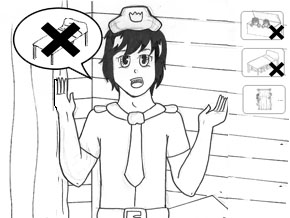
\includegraphics[scale=2.5]{OTL25.jpg}

\Bislama{Ale Lisa hemi se: \enquote{Christine hemi no bin kakae red yam blong yu, Mary! Ros nomo hemi spoilem yu!}}
\English{Then she says: \enquote{Christine didn't eat your red yam! It was Rose!}}

\Annotate
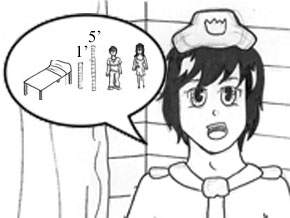
\includegraphics[scale=2.5]{OTL26.jpg}

\Bislama{Ale Lisa hemi se: \enquote{Christine hemi no bin kakae red yam blong yu, Mary! Ros nomo hemi spoilem yu!}}
\English{Then she says: \enquote{Christine didn't eat your red yam! It was Rose!}}

\Annotate
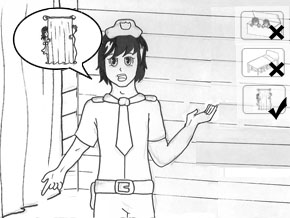
\includegraphics[scale=2.5]{OTL27.jpg}

\Bislama{Ale Lisa hemi se: \enquote{Christine hemi no bin kakae red yam blong yu, Mary! Ros nomo hemi spoilem yu!}}
\English{Then she says: \enquote{Christine didn't eat your red yam! It was Rose!}}

\Annotate
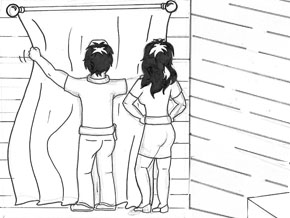
\includegraphics[scale=2.5]{OTL28.jpg}

\Bislama{Ale Lisa hemi se: \enquote{Christine hemi no bin kakae red yam blong yu, Mary! Ros nomo hemi spoilem yu!}}
\English{Then she says: \enquote{Christine didn't eat your red yam! It was Rose!}}

\Annotate
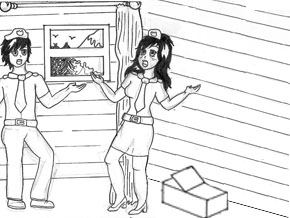
\includegraphics[scale=2.5]{OTL29.jpg}

\Bislama{Ale Lisa hemi se: \enquote{Christine hemi no bin kakae red yam blong yu, Mary! Ros nomo hemi spoilem yu!}}
\English{Then she says: \enquote{Christine didn't eat your red yam! It was Rose!}}

\Annotate
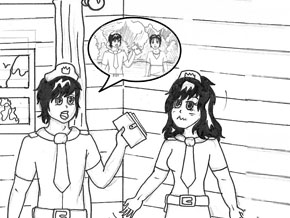
\includegraphics[scale=2.5]{OTL30.jpg}

\Bislama{Ale Lisa hemi se: \enquote{Christine hemi no bin kakae red yam blong yu, Mary! Ros nomo hemi spoilem yu!}}
\English{Then she says: \enquote{Christine didn't eat your red yam! It was Rose!}}

\Annotate


\end{document}
